%
% m-multipole.tex
%
% (c) 2017 Prof Dr Andreas Müller, Hochschule Rapperswil
%
\section{Multipolentwicklung}
\rhead{Multipolentwicklung}
In Abschnitt~\ref{skript:multipol:1dimbeispiel} haben wir ein
eindimensionales Beispiel untersucht, und mussten nach dem Potential
eines Dipols mit Vermutungen operieren, wie die weiteren Terme aussehen
müssten.
In diesem Abschnitt arbeiten wir in drei Dimensionen, und sind daher
in der Lage, kompliziertere Konfigurationen von Ladungen zu
konstruieren, und damit auch die späteren Terme der Entwicklung
genauer zu untersuchen.


\subsection{Dipol}
\begin{figure}
\centering
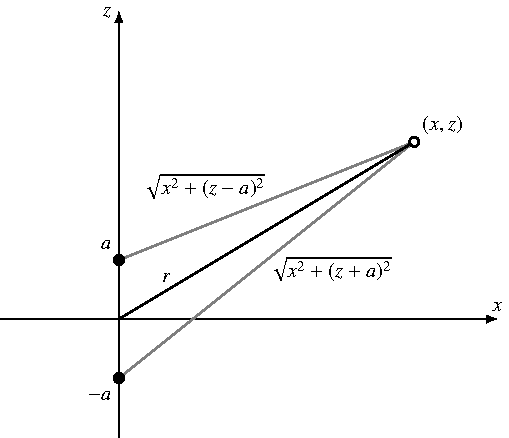
\includegraphics{chapters/tikz/dipol2.pdf}
\caption{Berechnung des Dipolpotentials 
\eqref{skript:multipol:dipol} in der $x$-$z$-Ebene
\label{skript:multipol:figure:dipol}}
\end{figure}
Wir betrachten das Feld eines Paares von entgegengesetzen Ladungen
in den Punkten $(0,0,a)$ und $(0,0,-a)$
(Abbildung~\ref{skript:multipol:figure:dipol}).
Der Einfachheit halber führen wir die Rechnung zunächst nur
in der $x$-$z$-Ebene durchführen und erst später mit Hilfe einer
vektoriellen Schreibweise auf drei Dimensionen erweitern.

Entlang der $z$-Achse kennen wir das Potential bereits aus
dem vorangegangenen Abschnitt.
Entlang der $x$-Achse verschwindet das Potential, denn die Punkte
auf der $x$-Achse sind von den beiden Ladungen gleich weit entfernt,
haben als entgegengesetzt gleiches Potential bezüglich beiden Ladungen
und damit totales Potential 0.

Wir betrachten jetzt das Potential im Punkt $(x,z)$, es ist
\begin{equation}
f(x,z)
=
\frac{q}{4\pi\varepsilon_0}
\biggl(
\frac{1}{\sqrt{x^2 + (z-a)^2}}
-
\frac{1}{\sqrt{x^2 + (z+a)^2}}
\biggr).
\label{skript:multipol:dipol}
\end{equation}
Offenbar müssen wir die Nenner besser verstehen, um diese Summe 
umformen zu können.
Speziell müssen wir die Abhängigkeit von der Entfernung
$r=\sqrt{x^2+z^2}$ vom Nullpunkt
und die Richtungsabhängigkeit voneinander trennen.
Dazu betrachten wir nur einen einzelnen Term
\[
\frac{1}{\sqrt{x^2+(z\pm a)^2}}
=
\frac{1}{\sqrt{x^2+z^2\pm 2az+a^2}}
=
\frac{1}{\sqrt{x^2+z^2}} \cdot \frac{1}{\sqrt{1+\frac{\pm 2az+a^2}{x^2+z^2}}}
=
\frac{1}{r} \cdot \frac{1}{\sqrt{1+\frac{\pm 2az+a^2}{r^2}}}
\]
Für grosse Werte von $r$ verschwindet der zweite Term in der Wurzel,
in erster Näherung verhält sich die Funktion daher wie $1/r$.
In den zwei Termen von \eqref{skript:multipol:dipol} hebt sich dieses
Verhalten jedoch weg, um die Funktion $f(x,z)$ zu verstehen, ist es
daher nötig, die Abweichungen von $1/r$ genauer zu verstehen.

Offenbar müssen wir Terme der Form
\begin{equation}
\frac{1}{\sqrt{1+t}}
=
(1+t)^{-\frac12}
\label{skript:multipol:wurzel}
\end{equation}
ausrechnen können, wobei wir später $t=(\pm2az+a^2)/r^2$ setzen wollen.

\subsubsection{Binomialreihe}
Die Taylor-Reihe der Funktion \eqref{skript:multipol:wurzel}
würde unser Problem lösen. 
Wir können die Reihe aber gleich für die
allgemeinere Funktionen
\begin{equation}
g(t)=(1+t)^\alpha
\end{equation}
mit beliebigem Exponenten bestimmen.

Dazu müssen die Ableitungen der Funktion $g(t)$ bestimmt werden
\begin{align*}
g'(t)
&=
\alpha(1+t)^{\alpha-1}
&
g'(0)&=\alpha
\\
g''(t)
&=
\alpha(\alpha-1)(1+t)^{\alpha-2}
&
g''(0)&=\alpha(\alpha-1)
\\
&\;\vdots
\\
g^{(n)}(t)
&=
\alpha(\alpha-1)(\alpha-2)\dots(\alpha-n+1) (1+t)^{\alpha -n}
&
g^{(n)}(0)&=\alpha(\alpha-1)(\alpha-2)\dots(\alpha -n +1)
\end{align*}
Der Term zur Potenz $n$ in der Taylor-Reihe von $g(t)$ ist
\[
\frac{\alpha(\alpha-1)(\alpha-2)\dots(\alpha-n+1)}{n!} t^n
\]
Wäre $\alpha$ eine ganze Zahl, dann sähe der Bruch
genau so aus wie der Binomialkoeffizient $\binom{\alpha}{k}$.
In Erweiterung der üblichen Definition des Binomialkoeffizienten
schreibt man auch für nicht ganzzahlige $\alpha$
\[
\binom{\alpha}{n}
=
\frac{\alpha(\alpha-1)(\alpha-2)\dots(\alpha-n+1)}{n!}.
\]
Mit dieser Schreibweise bekommen wir die Taylorreihe
\[
(1+t)^\alpha=\sum_{k=1}^\infty \binom{\alpha}{k} t^k
\]
für die Funktion $(1+t)^\alpha$.
Sie heisst die {\em Binomialreihe} und ist konvergent für $|t|<1$.
\index{Binomialreihe}

\subsubsection{Der Fall $\alpha=-\frac12$}
Wir betrachten die Binomialreihe für den Fall $\alpha=-\frac12$, der
uns im Zusammenhang mit \eqref{skript:multipol:dipol} speziell
interessiert.
Der Term zur Potenz $n$ ist
\begin{equation}
\frac{
\bigl(-\frac12\bigr)
\bigl(-\frac32\bigr)
\bigl(-\frac52\bigr)
\cdots
\bigl(-\frac{2n+1}2\bigr)}{n!} t^n
=
(-1)^n \frac{1\cdot 3\cdot 5 \cdots (2n + 1)}{2^n\cdot 1\cdot 2\cdot 3\cdots n}
=
(-1)^n \frac{1\cdot 3\cdot 5 \cdots (2n+1)}{2\cdot 4\cdot 6\cdots (2n)}
\label{skript:multipol:koeffizienten}
\end{equation}
Die zugehörige Potenzreihe ist daher
\[
\frac1{\sqrt{1+t}}
=
1-\frac12t+\frac3{8}t^2-\frac{15}{48}t^3+\frac{105}{354}t^4-\dots
\]
%deren Koeffizienten man auch faktorisieren und damit etwas
%Für 
%\[
%\frac1{\sqrt{1+t}}
%=
%1-\frac12 t
%+ \frac12\frac32\frac12 t^2
%- \frac 12\frac32\frac 52\frac1{3!} t^3
%+ \frac 12\frac32\frac 52\frac72\frac1{4!} t^4
%- \frac 12\frac32\frac 52\frac72\frac92\frac1{5!} t^4
%+\dots
%\]

Wir verwenden die binomische Reihe jetzt, um das Dipolpotential
zu berechnen.
Setzen wir 
\[
t=\frac{\pm 2az+a^2}{r^2}
\]
in der binomischen Reihe, erhalten wir
\[
\frac{1}{\sqrt{1+\frac{\pm 2az+a^2}{r^2}}}
=
1-\frac12\frac{\pm 2az+a^2}{r^2}
+
\frac38 \biggl(\frac{\pm 2az+a^2}{r^2}\biggr)^2+\dots
\]
und für das Dipolpotential $f(x,z)$ gemäss \eqref{skript:multipol:wurzel}
\begin{align*}
f(x,z)
&=
\frac{q}{4\pi\varepsilon_0 r}
\biggl(
1-\frac12\frac{-2az+a^2}{r^2} + \frac38 \biggl(\frac{-2az+a^2}{r^2}\biggr)^2+\dots
\biggr)
\\
&\qquad
-
\frac{q}{4\pi\varepsilon_0 r}
\biggl(
1-\frac12\frac{2az+a^2}{r^2} + \frac38 \biggl(\frac{2az+a^2}{r^2}\biggr)^2+\dots
\biggr)
\\
&=
-\frac{2aq}{4\pi\varepsilon_0r^3}z + \dots
\end{align*}
Wenn die beiden Ladungen näher zusammen rücken, wenn also $a\to 0$,
dann verschwindet das Potential.
Wenn wir das Potential weiterhin sehen wollen, müssen wir den Betrag
der Ladungen entsprechend vergrössern.
Wenn wir $a$ gegen $0$ gehen lassen, lassen wir gleichzeit die Ladung
$q$ grösser werden, so dass das Produkt $d=2qa$ gleich bleibt.
Mit dieser Konvention wird das Dipolpotential
\begin{equation}
f(x,z) = -\frac{d}{4\pi\varepsilon_0 r^2}\frac{z}{r}+\dots
\label{skript:multipol:dipolpotential}
\end{equation}
Darin haben wir statt $z$ den Bruch $z/r$ abgespalten, da dieser
entlang eines vom Nullpunkt ausgehenden Strahls vom Zentrum jeweils
konstant ist.
Wir haben daher das Potential in Faktoren aufgeteilt, die verschiedene
geometrische Bedeutung haben.
Der Faktor $1/r^2$ beschreibt, wie das Potential mit der Entfernung abnimmt.
Der Faktor $z/r$ beschreibt, wie das Potential von der Richtung im
Bezug auf die $z$-Achse abhängt.
Die übrigen Faktoren beschreiben, wie das Potential aus dem Dipolmoment
$d$ erzeugt wird.

\subsubsection{Vektorschreibweise}
Das Dipolpotential kann besonders elegant geschrieben werden, wenn
wir das skalare Dipolmoment $d$ durch einen Vektor $\vec{d}$ ersetzen.
In der Formel~\eqref{skript:multipol:dipolpotential}
für das Dipolpotential brauchen wir die $z$-Koordinate
des Punktes.
Diese können wir als das Skalarprodukt mit dem Standardbasisvektor
in $z$-Richtung bekomen.
Wenn wir also
\[
\vec{d}=\begin{pmatrix}0\\0\\d\end{pmatrix}
\]
setzen, dann können wir das Dipolpotential vektoriell als
\begin{equation*}
f(\vec{r})
=
-
\frac{1}{4\pi\varepsilon_0r^2} \frac{\vec{d}\cdot\vec{r}}{r}
\end{equation*}
geschrieben werden.
In dieser Form ist das Dipolpotential für jede beliebige Orientierung
des Dipolmomentes verwendbar.
In Abbildung~\ref{chapter:multipol:dipolniveaux} sind die Niveaulinien
des Dipolpotentials dargestellt für ein Dipolmoment, welches zur
$z$-Achse parallel ist..

Der Dipolterm geht für $r\to\infty$ wie $r^{-2}$ gegen $0$, also
deutlich schneller als das Potential einer Punktladung.

\begin{figure}
\centering
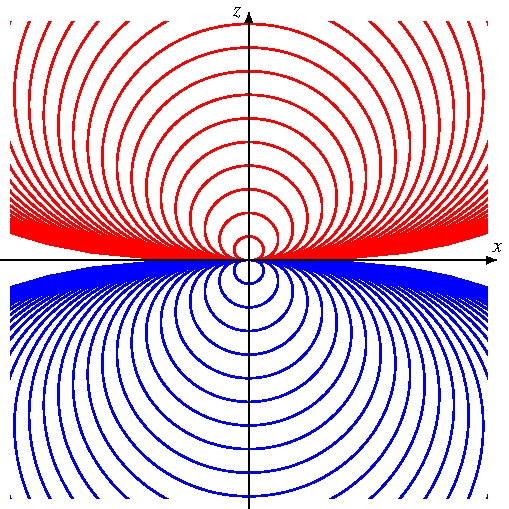
\includegraphics{chapters/tikz/dipol3.pdf}
\caption{Niveaulinien des Dipolpotentials für ein Dipolmoment
parallel zur $z$-Achse
\label{chapter:multipol:dipolniveaux}}
\end{figure}

\subsection{Quadrupol}
Wie in der eindimensionalen Situation vermuten wir, dass sich
das Potential komplizierterer Ladungsverteilungen ebenfalls durch
eine Reihe darstellen lässt, deren nächster Term von der Form
\begin{equation}
\frac1{4\pi\varepsilon_0}\cdot\frac{1}{r^5} p(\vec{r},\vec{r})
\label{skript:multipol:quadropolterm}
\end{equation}
sein muss.
Darin ist $p$ ein Ausdruck, der in beiden Argumenten linear ist.

Schreiben wir die Koordinaten als $(x_1,x_2,x_3)$, dann wird 
sich $p$ in der Form
\begin{equation}
\sum_{k,l=1}^3 Q_{kl}x_kx_l
\label{skript:multipol:qsumme}
\end{equation}
schreiben lassen.
Allerdings kann nicht jede beliebige Matrix zugelassen werden, 
da ja nur die Abweichungen vom Dipolmoment erfasst werden sollen.

\subsubsection{Symmetrie}
In der Summe~\eqref{skript:multipol:qsumme} kommt jeder Term
$x_kx_l$ mit $k\ne l$ zweimal vor, jeweils mit Koeffizient $Q_{kl}$
und $Q_{lk}$.
Die Summe kann daher auch geschrieben werden als
\[
\sum_{k,l=1}^3 Q_{kl}x_kx_l
=
\sum_{k=1}^3 \sum_{l=1}^{k-1} (Q_{kl}+Q_{lk})x_kx_l
+
\sum_{k=1}^3 Q_{kk}x_k^2
=
\sum_{k,l=1}^3 \frac12(Q_{kl}+Q_{lk}) x_kx_l.
\]
Die Matrix $\tilde Q_{kl}=\frac12(Q_{kl}+Q_{lk})$ führt also auf den
gleichen Quadrupolterm, aber mit einer symmetrischen Matrix $\tilde Q_{kl}$.
Es ist daher keine Einschränkung anzunehmen, dass $Q_{kl}$ symmetrisch ist.

\subsubsection{Spurbedingung}
Nimmt man für $Q$ die Einheitsmatrix, dann erhält man einfach nur
\[
\sum_{k,l=1}^3 Q_{kl}x_kx_l=\sum_{i=1}^3 x_i^2 = \vec{r}\cdot\vec{r}=r^2,
\]
der Quadrupol-Term wird also 
\[
\frac1{4\pi\varepsilon_0}\cdot\frac{1}{r^3},
\]
was keine Richtungsabhängigkeit mehr enthält und wir daher erwarten
würden, dass diese Art von Abhängigkeit bereits im ersten Term 
der Multipolreihe enthalten war.
Man kann dies zum Beispiel dadurch erreichen, dass die Matrix $Q$ 
verschwindende Spur haben soll, also $\operatorname{Spur}Q=0$.

\begin{figure}
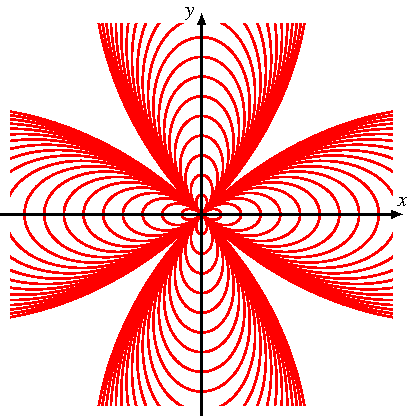
\includegraphics{chapters/tikz/quadrupol.pdf}
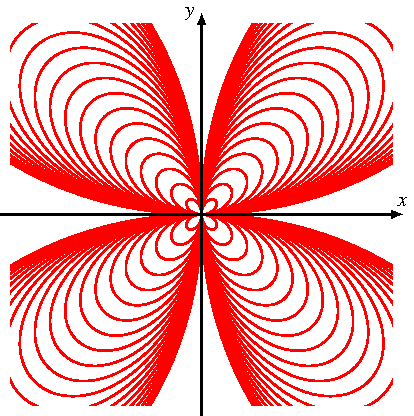
\includegraphics{chapters/tikz/quadrupol1.pdf}
\caption{Niveaulinien des Potentials eines Quadrupols.
Die $Q$-Matrizen sind 
$Q^{(1)}$ für das linke Bild und $Q^{(2)}$
für das rechte Bild
gemäss \eqref{skript:multipol:qmatrix}.
\label{chapter:multipol:quadrupolniveaux}}
\end{figure}

\begin{figure}
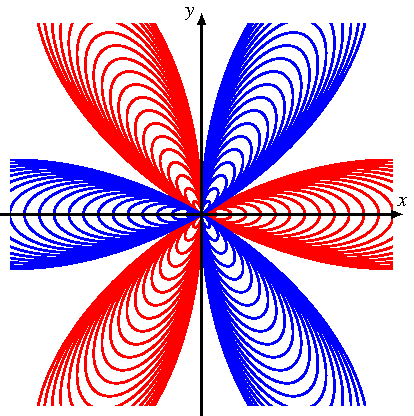
\includegraphics{chapters/tikz/hexapol.pdf}
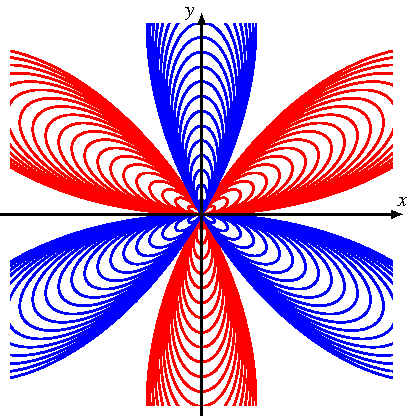
\includegraphics{chapters/tikz/hexapol1.pdf}
\caption{Niveaulinien des Potentials eines Hexapols.
Links der Fall $q_0=1,q_1=0$, rechts $q_0=0,q_1=1$.
\label{chapter:multipol:hexapolniveaux}}
\end{figure}

\subsubsection{Quadrupolterme in zwei Dimensionen}
In zwei Dimensionen gibt es nur zwei linear unabhängige Matrizen, die die
beiden eben genannten Bedingungen erfüllen, nämlich
\begin{align}
Q^{(1)}&=\begin{pmatrix}1&0\\0&-1\end{pmatrix}
&&\text{und}&
Q^{(2)}&=\begin{pmatrix}0&1\\1&0\end{pmatrix}.
\label{skript:multipol:qmatrix}
\\
\intertext{%
Schreibt man in Polarkoordinaten $x_1=r\cos\varphi$ und $x_2=r\sin\varphi$,
dann ist der Quadrupolterm in den beiden Fällen
}
&r^2(\cos^2\varphi-\sin^2\varphi)=r^2\cos 2\varphi
&&\text{bzw.}&
&2r^2\cos\varphi\sin\varphi.
\notag
\\
\intertext{%
Die Niveaulinien haben dann in Polarkoordinaten die Gleichungen
}
r&=\sqrt[3]{c \cos2\varphi}
&&\text{bzw.}&
r&=\sqrt[3]{c \sin2\varphi}.
\label{skript:multipol:quadrupolpolar}
\end{align}
In der Abbildung~\ref{chapter:multipol:quadrupolniveaux} sind die die
beiden Funktionen von
\eqref{skript:multipol:quadrupolpolar} dargestellt.
Man erkennt, dass $Q^{(2)}$ ein gegenüber $Q^{(1)}$ um $45^\circ$ verdrehtes
Potential ergibt.
Linear-Kombination von $Q^{(1)}$ und $Q^{(2)}$ entsprechen um beliebige
Winkel verdrehte Quadrupolpotentiale.

\subsubsection{Berechnung des Quadrupolterms}
Die konkrete Berechnung des Quadrupolanteils, also der Koeffizienten
$Q_{kl}$, ist etwas mühsam, wir geben hier nur das Resultat an.
Man findet
\cite{skript:brandtdahmen}
\[
Q_{kl}
=
\int_{\mathbb R^3}
\varrho(\vec{r}) \cdot (3x_kx_l-r^2\delta_{kl})
\,dx_1\,dx_2\,dx_3.
\]
Das Wachstum des Quadrupolterms~\eqref{skript:multipol:quadropolterm}
ist also von der Ordnung $r^{-3}$.
Auch dieser Term geht wieder einer Potenz schneller gegen $0$ als der
Dipolterm.

\subsection{Höhere Multipole}
Die Entwicklung Entwicklung in Dipol und Quadrupol lässt sich noch
weiter führen.
Dabei werden sukzessive Terme entstehen, die immer schneller gegen $0$
gehen, für grosse Entfernung vom Nullpunkt also immer weniger von
Bedeutung sein werden.
Die Darstellung dieser höheren Multipole wird allerdings zunehmen
schwierig. 
Der nächste Term nach dem Quadrupolterm, der Oktupolterm, müsste die Form
\begin{equation}
\frac1{4\pi\varepsilon_0}\frac{p(\vec r)}{r^7}
\label{skript:multipol:7ord}
\end{equation}
haben, wobei der Zähler $p(\vec r)$ eine Grösse dritter Ordnung in
den Koordinaten sein müsste.
Er wird also durch ein homogenes Polynom dritten Grades in den Koordinaten
$x$, $y$ und $z$ beschrieben.
Der Term~\eqref{skript:multipol:7ord} geht wie $r^{-4}$ gegen Null,
also erneut eine Potenz schneller als der Quadrupolterm.

Ganz allgemein erwarten wir, dass der $n$-te Multipolterm von der Form
\[
\frac{1}{4\pi\varepsilon_0} \frac{p(\vec r)}{r^{2n+1}}
\]
sein muss.
Darin ist $p(\vec r)$ ein Polynom vom Grade $n$ in den Koordinaten
des Ortsvektors $\vec r$.
Die Polynomkoeffizienten lassen sich als Grösse $Q_{i_1i_2\dots i_n}$
mit $n$ Indizes schreiben,
der $2^n$-Pol-Term wir zu der Summe
\begin{equation}
\frac{1}{4\pi\varepsilon_0}
\sum_{i_1,\dots,i_n} Q_{i_1\dots i_n} x_{i_1}\cdots x_{i_n}.
\label{skript:multipol:npolterm}
\end{equation}
Wie für die Quadrupolkoeffizienten können wir vollständige Symmetrie
der $Q_{i_1\dots i_n}$ annehmen, eine Vertauschung zweier beliebiger
Inidzes ändert nichts.
Ausserdem können wir annehmen, dass jede Summe über zwei gleichgesetzte
Indizes $0$ ergibt, denn eine solche Summe entspricht einem $2^{n-2}$-Pol-Term,
die wir im $2^n$-Pol-Term nicht darstellen wollen.

\subsubsection{Multipole in zwei Dimensionen}
In zwei Dimensionen lassen sich die $Q$ und die Multipolterme vollständig
ausrechnen.
Dazu beachten wir, dass wegen der vollständigen Symmetrie alle 
$Q_{i_1\dots i_n}$ mit der gleichen Anzahl Index $2$ gleich sein
müssen.
Wir können sie daher $q_k$ abkürzen, es ist also zum Beispiel
$Q_{1\dots 1}=q_0$ und $Q_{2\dots 2}=q_n$.

Die Spurbedingungen sagt dann, dass
\[
Q_{i_1\dots 11\dots i_n}
+
Q_{i_1\dots 22\dots i_n}
=
0
\qquad\Rightarrow\qquad
Q_{i_1\dots 11\dots i_n}
=-
Q_{i_1\dots 22\dots i_n}
\qquad\Rightarrow\qquad
q_{k+2}=-q_k
\]
Es gibt also nur zwei linear unabhängige $Q_{i_1\dots i_n}$, die durch
die Wahl von $q_0$ bzw.~$q_1$ festgelegt sind, die wir ohne Einschränkung
$1$ setzen dürfen.

Für die Berechnung des Multipolterms müssen wir wissen, wieviele Terme 
mit Koeffizient $q_k$ jeweils vorkommen.
Es gbit $\binom{n}{k}$ Koeffizienten $Q_{i_1\dots i_n}$ mit genau $k$
Indizes $2$.
Damit können wir jetzt die Multiplausdrücke berechnen:
\begin{align*}
q_0&=1, q_1=0
&
&\Rightarrow&
\frac{1}{4\pi\varepsilon_0}
\sum_{\text{$k$ gerade}} (-1)^{\frac{k}2}\binom{n}{k}
	\cos^{n-k}\varphi \sin^k\varphi
&=
\frac{1}{4\pi\varepsilon_0}
\cos n\varphi,
\\
q_0&=0, q_1=1
&
&\Rightarrow&
\frac{1}{4\pi\varepsilon_0}
\sum_{\text{$k$ ungerade}} (-1)^{\frac{k-1}2}\binom{n}{k}
	\cos^{n-k}\varphi \sin^k\varphi
&=
\frac{1}{4\pi\varepsilon_0}
\sin n\varphi.
\end{align*}
Die Multipolterme sind also durch trigonometrische Funktionen der
vielfachen Winkel gegeben.
Für den Fall $n=3$ sind die zugehörigen Niveauflächen in
Abbildung~\ref{chapter:multipol:hexapolniveaux} dargestellt.

\section{Richtungsabhängigkeit und Entfernungsbhängigkeit}
In den Termen \eqref{skript:multipol:npolterm} der Multipolentwicklung
ist die Richtungsabhängigkeit noch nicht von der Entfernungsabhängigkeit
getrennt.
Die Koordinaten $x_i$ wachsen mit zunehmender Entfernung ebenfalls an.
Wenn wir also wie in der Einleitung versprochen Richtung und Entfernung
trennen wollen, dann müssen wir die Terme als Funktionen von $r$ für die
Entfernung und den Komponenten $x/r$, $y/r$ und $z/r$ des Einheitsvektors
der Richtung ausdrücken.
Dafür stehen aber im Nenner $1/r^{2n+1}$ genügend Faktoren $r$ zur Verfügung.

Ausdgedrückt durch die Quotienten $x_k/r$ wird die Multipolentwicklung
also zu
\begin{align}
f(\vec r)
&=
\frac{1}{4\pi\varepsilon_0}
\biggl(
q
\frac{1}{r}
+
\frac{1}{r^2} \frac{\vec{d}\cdot\vec{r}}{r}
+
\frac{1}{r^3} \sum_{k,l}Q_{kl}\frac{x_k}{r}\frac{x_l}{r}
+
\frac{1}{r^4} \sum_{k,l,j}Q_{klj}\frac{x_k}{r}\frac{x_l}{r}\frac{x_j}{r}
+
\dots
\biggr)
\notag
\\
&=
\frac{1}{4\pi\varepsilon_0}
\biggl(
\frac{1}{r} Q
+
\frac{1}{r^2} \sum_{k}Q_k \frac{x_k}{r}
+
\frac{1}{r^3} \sum_{k,l}Q_{kl}\frac{x_k}{r}\frac{x_l}{r}
+
\frac{1}{r^4} \sum_{k,l,j}Q_{klj}\frac{x_k}{r}\frac{x_l}{r}\frac{x_j}{r}
+
\dots
\biggr).
\label{skript:multipol:allgemein}
\end{align}
Allen Termen ist gemeinsam, dass sie die Abhängigkeit des Potentials in einen
aus physikalischen Gründen plausiblen radialen Teil der Form $r^{-k}$
und einen richtungsabhängigen Teil aufteilen.
Die reine Richtungsabhängigkeit wird dadurch ausgedrückt, dass
die einzelnen Summen in \eqref{skript:multipol:allgemein}
nur von den Quotienten $x/r$, $y/r$ und $z/r$ abhängt, und zwar
als Polynom vom Grad $k-1$.



